\documentclass[11pt]{article}
\title{Lenses}
\author{https://github.com/heptagons/lenses}
\date{2023/12/30}

\usepackage{graphicx}

\usepackage[margin=0.75in]{geometry}
\usepackage{float} % {figure}{H}
\usepackage{amsmath} % \dfrac


%\usepackage{amssymb}
%\usepackage{subcaption}

\def\mathbi#1{\textbf{\em #1}}

\begin{document}

\maketitle
\begin{abstract}
Lenses are equilateral hexagons resembling concave and convex optical lenses. The hexagons consecutive six internal angles are $(\theta_1,\theta_2,\theta_3,\theta_1,\theta_2,\theta_3)$ where $\theta_1=X\theta_0$, $\theta_2=Y\theta_0$, and $\theta_3=Z\theta_0$ where $\theta_0 = 2\pi/S$ is the base angle of symmetry $S = X + Y + Z$.
\end{abstract}

\section{Lenses}

\section{Symmetry $5$}

Symmetry $5$ uses as base the angle $\beta = \dfrac{2\pi}5$. Includes the rhombi $(\mathbi{b},\mathbi{c})$ and the lenses $(\mathbi{B},\mathbi{C})$.


\subsection{Rhombi $(\mathbi{b},\mathbi{c})$}

\begin{figure}[H]
\centering
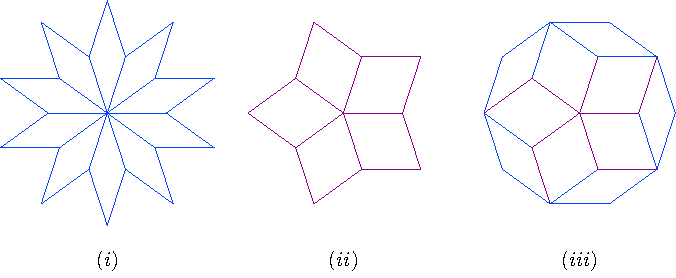
\includegraphics[scale=1.1]{bc/rhombi}
\caption{Rhombi $(\mathbi{b},\mathbi{c})$.}
\label{fig:bc-rhombi}
\end{figure}

\begin{table}[H]
\begin{center}
\begin{tabular}{|c|c c|}
\hline
Rhombus & $\theta_1$ & $\theta_2$ \\ %[1ex]
\hline\
$\mathbi{b}$ & $\beta/2$ & $4\beta/2$ \\[0.5ex] \hline
%& \\[-1ex]
$\mathbi{c}$ & $2\beta/2$ & $3\beta/2$ \\[0.5ex] \hline
%\hline
%\hline
\end{tabular}
\caption{Rhombi $(\mathbi{b},\mathbi{c})$ internal angles $\theta_1 + \theta_2 = \pi$ where $\beta = 2\pi/5$.} 
\label{tbl:bc-angles}
\end{center}
\end{table}

Figure \ref{fig:bc-rhombi} show rhombi $(\mathbi{b},\mathbi{c})$. 
Inspecting the figures we get these areas:
Star at $(i)$ is $10\mathbi{b}$, star at $(ii)$ is $5\mathbi{c}$ and 
regular pentagon at $(iii)$ is $5\mathbi{b} + 5\mathbi{c}$. Table \ref {tbl:bc-angles} show the angles.

\begin{figure}[H]
\centering
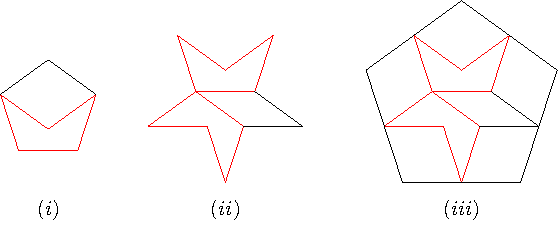
\includegraphics[scale=1.1]{bc/penta}
\caption{Regular pentagon and pentagram. Concave pentagon (in red).}
\label{fig:bc-penta}
\end{figure}

Figure \ref{fig:bc-penta} show regular pentagon and pentagram dissected with rhombi $(\mathbi{b},\mathbi{c})$ and a concave pentagon (in red). We calculate the areas of the regular pentagon $P_1$ at $(i)$ and pentagram $P_G$ at $(ii)$ in function of rhombi $(\mathbi{b},\mathbi{c})$. Let $x$ be the concave pentagon area. From the figures we note pentagon $P_2$ at $(iii)$ is double the side and then four times the area of pentagon $P_1$. From the figures we note the area of $P_1$ is $x + \mathbi{c}$ and the area of $P_2$ is $2x + \mathbi{b} + 5\mathbi{c}$, so we compare the pentagons and solve for $x$ to get:
\begin{align}
4P_1 &= P_2 \nonumber\\
4(x + \mathbi{c}) &= 2x + \mathbi{b} + 5\mathbi{c} \nonumber\\
x &= \frac{\mathbi{b} + \mathbi{c}}2
\end{align}
Then the areas of the pentagon and the pentagram are:
\begin{align}
P_1 &= x + \mathbi{c} 
 = \frac{\mathbi{b} + \mathbi{c}}2 + \mathbi{c}
 = \frac{\mathbi{b} + 3\mathbi{c}}2 \\
P_G &= 2x + \mathbi{b}
 = \frac{2(\mathbi{b} + \mathbi{c})}2 + \mathbi{b}
 = 2\mathbi{b} + \mathbi{c}
\end{align}

\subsection{Lenses $(\mathbi{B},\mathbi{C})$}

\begin{figure}[H]
\centering
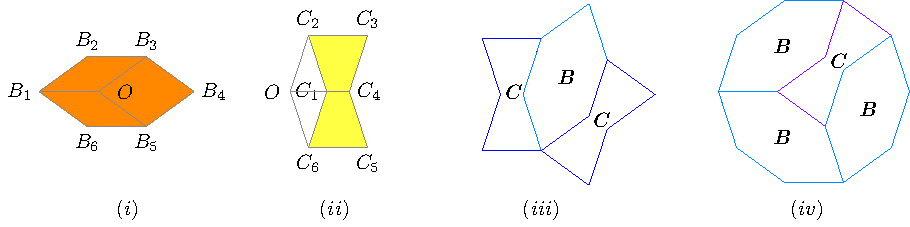
\includegraphics[scale=1.1]{bc/hexagons}
\caption{Lenses $(\mathbi{B}, \mathbi{C})$.}
\label{fig:bc-hexagons}
\end{figure}

\begin{table}[H]
\begin{center}
\begin{tabular}{|c|c c c|}
\hline
Rhombus & $\theta_1$ & $\theta_2$ & $\theta_3$ \\ %[1ex]
\hline\
$\mathbi{B}$ & $\beta$ & $2\beta$ & $2\beta$ \\[0.5ex] \hline
%& \\[-1ex]
$\mathbi{C}$ & $\beta$ & $\beta$ & $3\beta$ \\[0.5ex] \hline
%\hline
%\hline
\end{tabular}
\caption{Lenses $(\mathbi{B},\mathbi{C})$ internal angles $\theta_1+\theta_2+\theta_3 = 2\pi$ where $\beta = 2\pi/5$.} 
\label{tbl:bc-lenses-angles}
\end{center}
\end{table}


Figure \ref{fig:bc-hexagons} show lenses $(\mathbi{B},\mathbi{C})$.
Figure $(i)$ show the lense $\mathbi{B}$ with perimeter $\overline{B_1...B_6}$ is formed adding two rhombi $\mathbi{b}$ and adding one rhombus $\mathbi{c}$ so its area is $2\mathbi{b} + \mathbi{c}$.
Figure $(ii)$ show the lense $\mathbi{C}$ with perimeter $\overline{C_1...C_6}$ is formed adding two rhombi $\mathbi{c}$ and substracting one rhombus $\mathbi{b}$ so its area is $2\mathbi{c} - \mathbi{b}$.
From the figures we see the area of star $(iii)$ is $\mathbi{B} + 2\mathbi{C} = 5\mathbi{c}$
and the area of regular decagon $(iv)$ is $3\mathbi{B} + \mathbi{C} = 5\mathbi{b} + 5\mathbi{c}$.

\section{Symmetry $7$}

Symmetry $7$ uses as base the angle $\gamma = \dfrac{2\pi}7$. Includes the rhombi $(\mathbi{d},\mathbi{f},\mathbi{e})$ and the lenses $(\mathbi{D},\mathbi{E},\mathbi{F})$.

\subsection{Rhombi $(\mathbi{d},\mathbi{e},\mathbi{f})$}

\begin{figure}[H]
\centering
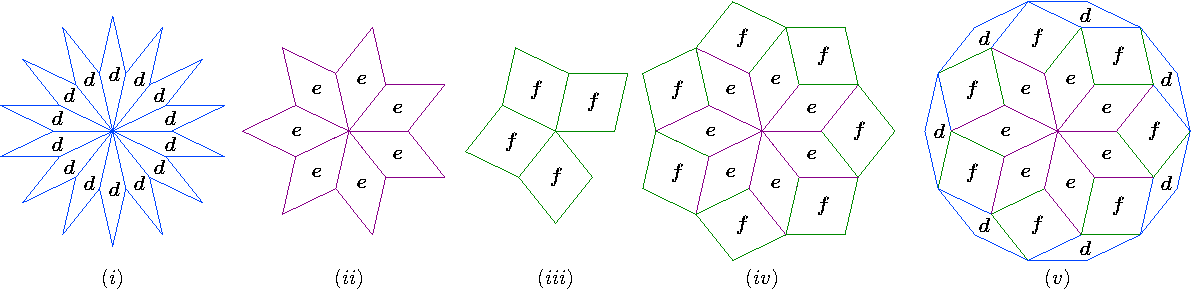
\includegraphics[scale=0.9]{def/rhombi}
\caption{Rhombi $(\mathbi{d},\mathbi{e},\mathbi{f})$.}
\label{fig:def-rhombi}
\end{figure}

\begin{table}[H]
\begin{center}
\begin{tabular}{|c|c c|}
\hline
Rhombus & $\theta_1$ & $\theta_2$ \\ %[1ex]
\hline\
$\mathbi{d}$ & $\gamma/2$ & $6\gamma/2$ \\[0.5ex] \hline
$\mathbi{e}$ & $2\gamma/2$ & $5\gamma/2$ \\[0.5ex] \hline
$\mathbi{f}$ & $3\gamma/2$ & $4\gamma/2$ \\[0.5ex] \hline
%\hline
%\hline
\end{tabular}
\caption{Rhombi $(\mathbi{d},\mathbi{e},\mathbi{f})$ internal angles $\theta_1 + \theta_2 = \pi$ where $\gamma = 2\pi/7$.} 
\label{tbl:def-angles}
\end{center}
\end{table}

Figure \ref{fig:def-rhombi} show rhombi $(\mathbi{d},\mathbi{e},\mathbi{f})$. 
Inspecting the figures we get these areas:
Star at $(i)$ is $14\mathbi{d}$, star at $(ii)$ is $7\mathbi{e}$ and irregular shape $(iii)$ is $4\mathbi{f}$. The star at $(iv)$ is $7(\mathbi{e} + \mathbi{f})$ and the regular 14-gon area is $7(\mathbi{d} + \mathbi{e} + \mathbi{f})$. Table \ref {tbl:def-angles} show the angles.


\end{document}
